\documentclass[11pt,letterpaper, leqno]{article}
\usepackage{latexsym}
\usepackage{amsmath}
\usepackage{amssymb}
\usepackage{amsthm}
\topmargin -0.25in
\textheight 8.5in
\oddsidemargin 0.0in
\textwidth 6.5in

\RequirePackage{amsthm,amsmath,amsfonts,amssymb}
%\RequirePackage[numbers]{natbib}
\RequirePackage[authoryear]{natbib}%% uncomment this for author-year citations
\RequirePackage[colorlinks,citecolor=blue,urlcolor=blue]{hyperref}%% uncomment this for coloring bibliography citations and linked URLs
\RequirePackage{graphicx}%% uncomment this for including figures

\usepackage{bbm}
\usepackage{natbib}
\usepackage{authblk}
\usepackage[english]{babel}
\bibliographystyle{abbrvnat}
\setcitestyle{authoryear,open={(},close={)}}

% For the algorithm table
\usepackage{algorithm,algcompatible,amsmath}
\DeclareMathOperator*{\argmax}{\arg\!\max}
\DeclareMathOperator*{\argmin}{\arg\!\min}
% https://tex.stackexchange.com/q/83169/5764
\algnewcommand\INPUT{\item[\textbf{Input:}]}%
\algnewcommand\OUTPUT{\item[\textbf{Output:}]}%
%

\newcommand{\ex}{{\bf\sf E}}            %% expectation
\newcommand{\bfp}{{\bf P}}
\newcommand{\bfr}{{\bf R}}
\newcommand{\Var}{{\rm Var}}            %% 
\newcommand{\Cov}{{\rm Cov}}            %% 
\newcommand{\calc}{{\cal C}}            %%
\newcommand{\cald}{{\cal D}} 
\newcommand{\calf}{{\cal F}}            %%
\newcommand{\call}{{\cal L}}            
\newcommand{\al}{\alpha}                %%
\newcommand{\bt}{\beta}                %%
\newcommand{\ga}{\gamma}                %% abbreviated
\newcommand{\dt}{\delta}                %% greek letters
\newcommand{\la}{\lambda}               %%
\newcommand{\ep}{\epsilon}              %%
\newcommand{\sig}{\sigma}               %%
\newcommand{\tri}{\triangle}
\newcommand{\om}{\omega}                %%
\newcommand{\ra}{\rightarrow}           %%
\newcommand{\lra}{\longrightarrow}
\newcommand{\Ra}{\Rightarrow}           %% arrows
\newcommand{\subs}{\subseteq}           %% subset or equal to
\newcommand{\eqdef}{\stackrel{\triangle}{=}}
\newcommand{\hY}{\hat{Y}}
\newcommand{\hp}{\hat{p}}
\newcommand{\hX}{\hat{X}}
\newcommand{\hy}{\hat{y}}
\newcommand{\hQ}{\hat{Q}}
\newcommand{\Zh}{\hat{Z}}
\newcommand{\hla}{\hat{\lambda}}
\newcommand{\starti}{\parindent0pt\it}  %% start an italic line
\newcommand{\startb}{\parindent0pt\bf}  %% start a boldface line
\newcommand{\tril}{\triangle^-}
\newcommand{\trir}{\triangle^+}
\newcommand{\trilr}{\triangle^{\pm}}
\newcommand{\realR}{{{\rm I}\;\!\!\!{\rm R}}}
\newcommand{\probP}{{{\rm I}\;\!\!\!{\rm P}}}
\newcommand{\filtF}{{{\rm I}\;\!\!\!{\rm F}}}
\newcommand{\expeE}{{{\rm I}\;\!\!\!{\rm E}}}
\newcommand{\noin}{{\noindent}}
\newcommand{\doty}{{\dot{y}}}
\newcommand{\doth}{{\dot{h}}}
\newcommand{\dotx}{{\dot{x}}}
\newcommand{\dotu}{{\dot{u}}}
\newcommand{\dotf}{{\dot{f}}}
\newcommand{\dotg}{{\dot{g}}}
\newcommand{\ddoty}{{\ddot{y}}}
\newcommand{\ddoth}{{\ddot{h}}}
\newcommand{\ddotx}{{\ddot{x}}}
\newcommand{\ddotf}{{\ddot{f}}}
%\newcommand{\Var}{{\mbox{Var}}}
%\newcommand{\Cov}{{\mbox{Cov}}}

\renewcommand{\Var}{\text{Var}}
\renewcommand{\P}{\mathbb{P}}
\newcommand{\R}{\mathbb{R}}
\newcommand{\E}{\mathbb{E}}
\newcommand{\Z}{\mathbb{Z}}
\renewcommand{\qed}{\quad \blacksquare}
\newcommand{\ind}{\mathbbm{1}}

\begin{document}
\begin{center}
{\bf \Large APMA1690: ~~Homework \# 3 ~~~(Due by 11pm Oct 5)}
\end{center}
\[\]
\medskip

\section{Review}

\begin{itemize}
    \item (\textbf{Multiplicative Congruential Generator}) \\
    For ``properly chosen" positive integers $m$ and $a$ (e.g., $m=2^{31}-1$ and $a=7^5$), we have the \href{https://en.wikipedia.org/wiki/Lehmer_random_number_generator}{multiplicative congruential generator} (MCG) presented by the following algorithm
\begin{algorithm}[H]
	\caption{: Multiplicative Congruential Generator}\label{algorithm: MCG}
	\begin{algorithmic}[1]
		\INPUT
        \noindent (i) positive integers $m$ and $a$; (ii) a \href{https://en.wikipedia.org/wiki/Random_seed}{seed} $s\in\{1,2,\ldots,m-1\}$; (iii) sample size $n$.
		\OUTPUT pseudo-random numbers $g(1), g(2), \ldots, g(n)$. (These numbers look like iid from $\operatorname{Unif}(\{1,2,\ldots,m-1\})$.)
		\STATE Initialization: $g(1)\leftarrow s$.
		\FORALL{$i=1, 2, \ldots, n-1$, }
        \STATE $g(i+1) \leftarrow (a\cdot g(i)$ mod $m$) = the remainder of $\frac{a\cdot g(i)}{m}$.
		\ENDFOR
		\end{algorithmic}
\end{algorithm}

The ``remainder" referred to in the algorithm above is the \href{https://en.wikipedia.org/wiki/Remainder}{remainder in integer division}.
    
\item (\textbf{Fundamental theorem for the ``\href{https://en.wikipedia.org/wiki/Inverse_transform_sampling}{inverse CDF method}"})\\ 
Let $F(t)$ be a CDF of interest. We define the function $G(u)$ on the open interval $(0,1)$ by
\begin{align}\label{Eq: def of G}
    G(u)=\inf\left\{ t\in\mathbb{R} \,:\, F(t)\ge u
    \right\}, \ \ \mbox{ for all }u\in(0,1),
\end{align}
where ``inf" denotes the \href{https://en.wikipedia.org/wiki/Infimum_and_supremum}{infimum} operation (you may view it as ``\href{https://en.wikipedia.org/wiki/Maximum_and_minimum}{min}" for simplicity). The function $G$ in Eq.~\eqref{Eq: def of G} is the ``\href{https://en.wikipedia.org/wiki/Cumulative_distribution_function#Inverse_distribution_function_(quantile_function)}{generalized inversion}" of $F$. Let $U$ be a random variable defined on the probability space $(\Omega,\mathbb{P})$ and following the \href{https://en.wikipedia.org/wiki/Continuous_uniform_distribution}{continuous uniform distribution} on $(0,1)$, i.e., $U\sim\operatorname{Unif}(0,1)$, and we define a new random variable $X$ by 
\begin{align*}
    X(\omega)=G\left(U(\omega)\right),\ \ \mbox{ for all }\omega\in\Omega.
\end{align*}
Then, the CDF of $X$ is the CDF $F(t)$ of interest. \\
\textbf{Remarks:} (i) For any given real number $0<u<1$, the notation ``$\left\{ t\in\mathbb{R} \,:\, F(t)\ge u
    \right\}$" denotes the collection of the real numbers $t$ such that $F(t)\ge u$. \\
    (ii) ``$\inf\left\{ t\in\mathbb{R} \,:\, F(t)\ge u
    \right\}$" denotes the smallest number in the collection $\left\{ t\in\mathbb{R} \,:\, F(t)\ge u
    \right\}$.\\
(iii) If the inverse $F^{-1}$ of $F$ exists, then $G=F^{-1}$.

\item Algorithm \ref{algorithm: Inverse CDF Method} algorithm provides the procedures for implementing the inverse CDF method.
\begin{algorithm}[ht]
	\caption{: Inverse CDF Method}\label{algorithm: Inverse CDF Method}
	\begin{algorithmic}[1]
		\INPUT
        \noindent (i) The CDF $F$ of interest; (ii) sample size $n$.
		\OUTPUT A sequence of iid (pseudo) random numbers $x_1, \ldots, x_n$ following the distribution $F$.
		\STATE Generate (pseudo) iid random variables $u_1, u_2,\ldots, u_n$ from $\operatorname{Unif}(0,1)$.
		\FORALL{$i=1,\ldots,n$, }
        \STATE Compute $x_i \leftarrow G(u_i)=\inf\{t\in\mathbb{R}: F(t)\ge u_i\}$.
		\ENDFOR
		\end{algorithmic}
\end{algorithm}

\end{itemize}

\newpage
\section{Problem Set}

\begin{enumerate}

\item This question helps you better understand the MCG. Let $g$ be the MCG in Algorithm \ref{algorithm: MCG}.
\begin{enumerate}
    \item (1 point) Write the computer code for the MCG as described in Algorithm \ref{algorithm: MCG} using your preferred programming language. Please include your code in your submission.
    
    \begin{center}
        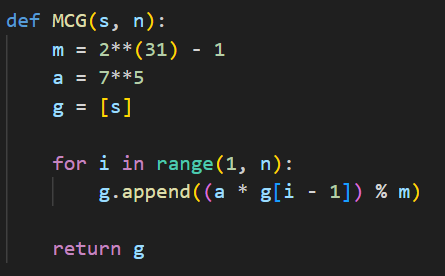
\includegraphics{Images/1A.png}
    \end{center}

    \item (1 point) Let $m=2^{31}-1$ and $a=7^5$. Initialize the seed by $g(1) \leftarrow 1690$ and generate $g(1),g(2),\ldots, g(10)$ using your code. Show all the ten numbers $g(1), g(2),\ldots, g(10)$ and the code for generating these numbers.
    
    \color{blue}
        \begin{center}
            \begin{tabular*}{1.2in}{|c c|}
                \hline
                $n$ & $g(n)$\\
                \hline
                1 & 1690\\
                2 & 28403830\\
                3 & 641801176\\
                4 & 2089489798\\
                5 & 254955595\\
                6 & 808809400\\
                7 & 88100290\\
                8 & 1085341247\\
                9 & 604240711\\
                10 & 23463114\\
                \hline
            \end{tabular*} \qquad 
            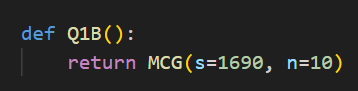
\includegraphics{Images/1B.png}
        \end{center}
    \color{black}

    \item (1 point) Let $m=2^{31}-1$ and $a=7^5$. Initialize the seed by $g(1) \leftarrow 1690$ and generate $g(1),g(2), \ldots, g(10000)$ using your code. Plot and show the histogram of the following 10000 values
    \begin{align*}
        \left\{\frac{g(1)}{m}, \frac{g(2)}{m}, \ldots, \frac{g(10000)}{m}\right\}.
    \end{align*}
    Show the code for generating this histogram.

    \color{blue}
        \begin{center}
            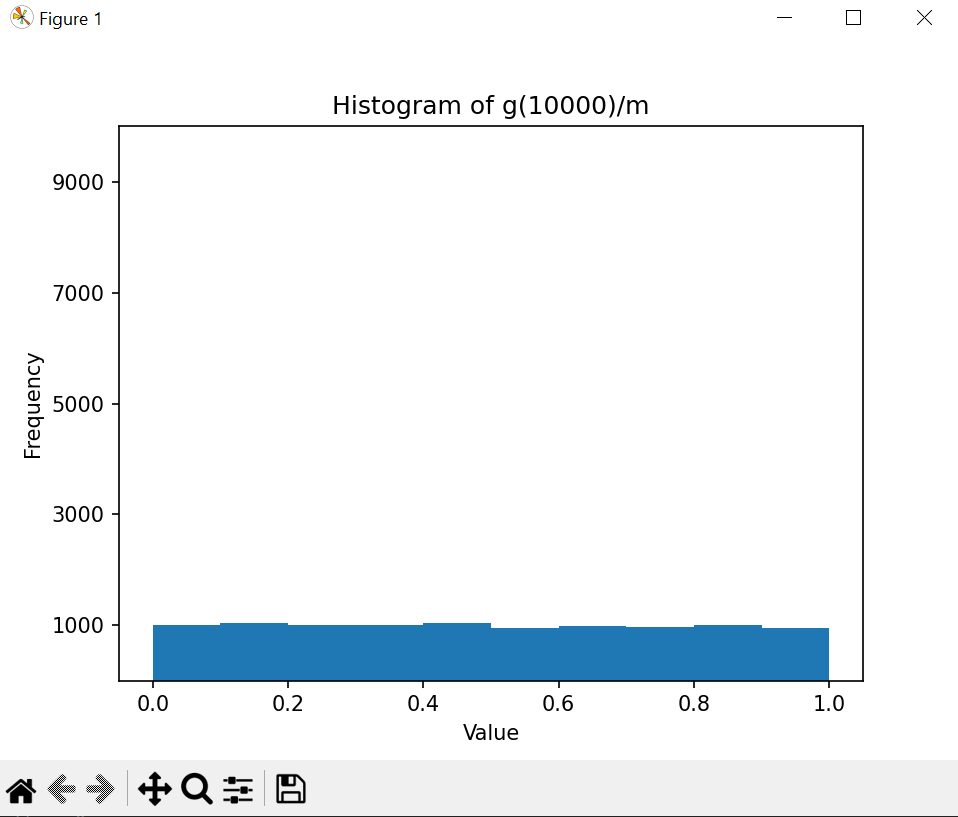
\includegraphics[width=0.8\textwidth]{Images/1C Histogram.png}
            
            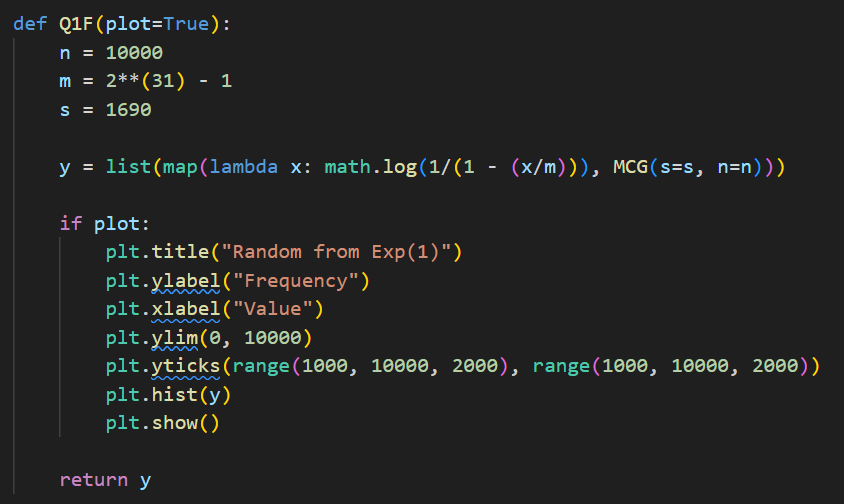
\includegraphics[width=0.8\textwidth]{Images/1C.png}
        \end{center}
    \color{black}

    \item (1 point) Please heuristically (rather than mathematically/rigorously) explain the relationship between the histogram you obtained in the preceding question and $\operatorname{Unif}(0,1)$.

    \color{blue}
        The sequence of random numbers $\left\{\frac{g(1)}{m}, \; \dots \;, \frac{g(n)}{m}\right\}$ ``look like'' random numbers taken iid from $\text{Unif}(0, 1)$. 
    \color{black}
    \vspace*{0.25in}
    \item (0.5 points) Let $F(t)=(1-e^{-t})\cdot\mathbbm{1}(t>0)$, which is the CDF of the  \href{https://en.wikipedia.org/wiki/Exponential_distribution}{exponential distribution} $\operatorname{Exp}(1)$. Compute an explicit express of the $G(u)$ defined in Eq.~\eqref{Eq: def of G} for all $0<u<1$.
    
    \color{blue}
        By the Fundamental Theorem of the Inverse CDF, we are looking for an explicit expression for 
        \[G(u) = \inf \{t \in \R: F(t) \geq u\} \quad \forall u\in (0, 1)\]
        Heuristically, we ask ``what is the smallest $t$ for which $F(t)$ is greater than or equal to $u$, for all $u \in (0, 1)$?''
        First, we observe 
        \[F(t) = (1 - e^{-t})\cdot \ind(t > 0) = \begin{cases}
            1 - e^{-t} \quad\;\, t > 0\\
            0 \qquad\qquad t \leq 0
        \end{cases}\]
        
        Immediately, we see that $G(u)$ is not defined for $t \leq 0$ and for $t > 0$:
        \begin{align*}
            G(u) &= \inf\{t \in \R: 1 - e^{-t} \geq u\}\\
            &= \inf\{t\in \R: 1 - u \geq e^{-t}\}\\
            &= \inf\{t\in \R: \log(1 - u) \geq -t\}\\
            &= \inf\{t\in \R: -\log(1 - u) \leq t\}\\
            &= \inf\{t\in \R: \log(\frac{1}{1 - u}) \leq t\}\\
            &= \boxed{\log(\frac{1}{1 - u})}
        \end{align*}
    \color{black}

    \item (0.5 points) Using the values $g(1),g(2), \ldots, g(10000)$ generated in the preceding question, plot and show the histogram of the following 10000 values
    \begin{align*}
        \left\{\log\left(\frac{1}{1-\frac{g(1)}{m}}\right), \log\left(\frac{1}{1-\frac{g(2)}{m}}\right), \ldots, \log\left(\frac{1}{1-\frac{g(10000)}{m}}\right)\right\},
    \end{align*}
    where ``$\log$" denotes the natural logarithm and $m=2^{31}-1$. Please heuristically (rather than mathematically/rigorously) explain the relationship between the histogram you obtained here and the probability density function of the  \href{https://en.wikipedia.org/wiki/Exponential_distribution}{exponential distribution} $\operatorname{Exp}(1)$.

    \color{blue}
        \begin{center}
            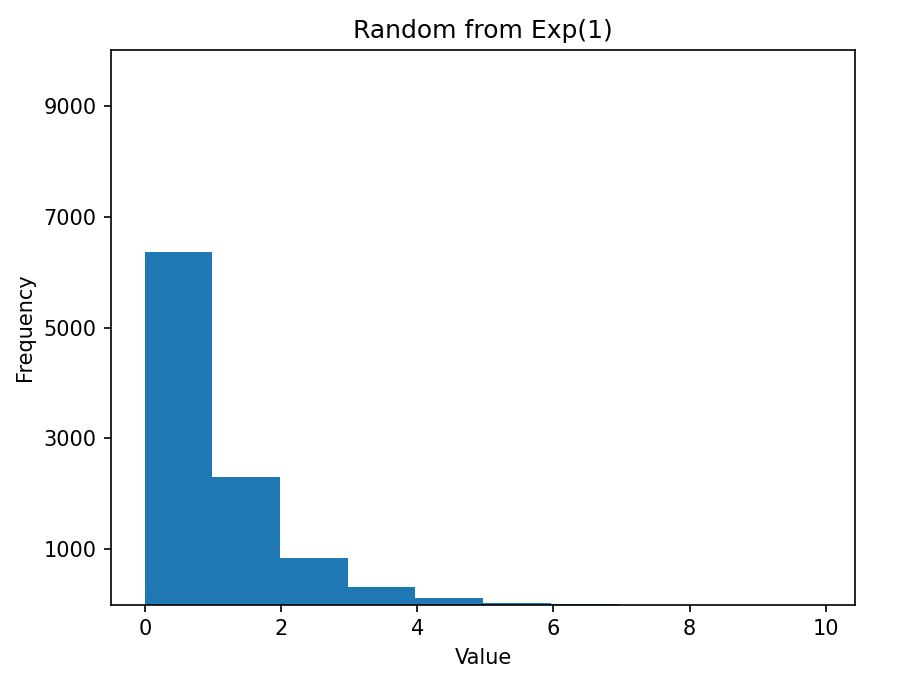
\includegraphics[width=0.6\textwidth]{Images/1F Histogram.png}

            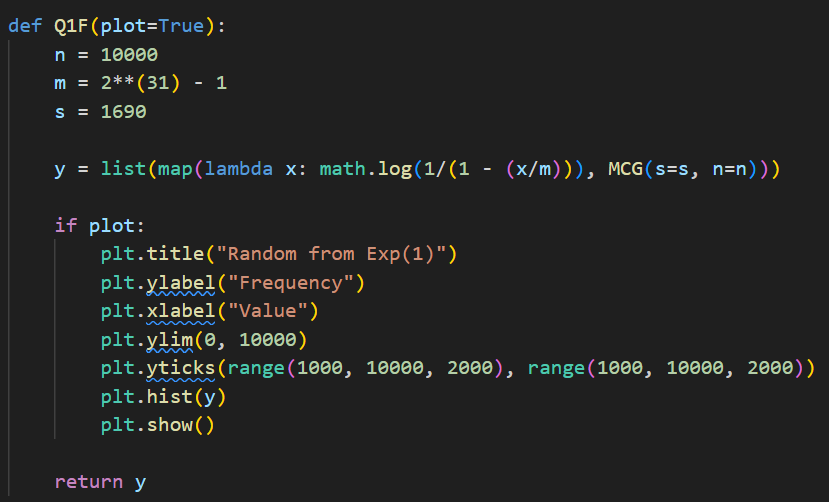
\includegraphics[width=0.6\textwidth]{Images/1F.png}

        \end{center}
        By the inverse CDF method, this sequence of values are random numbers which ``look like'' random numbers generated iid from the distribution $\text{Exp}(1)$.
    \color{black}
\end{enumerate}

\pagebreak
\item Let $X$ be a random variable defined on the probability space $(\Omega,\mathbb{P})$, and $X$ satisfies 
\begin{align*}
    \mathbb{P}\left\{ \omega\in\Omega \,:\, X(\omega)=i\right\} = \frac{1}{n}, \ \ \mbox{ for all }i=1,2,\ldots,n.
\end{align*}
where $n$ is a given positive integer. Define a new random variable $Y$ by
    \begin{align*}
        Y(\omega)=\frac{X(\omega)}{n},\ \ \mbox{ for all }\omega\in\Omega.
    \end{align*}
\begin{enumerate}
    \item (0.5 point) Show that the CDF of $Y$ is the following
\begin{align}\label{eq: def of Fm}
    \begin{aligned}
        F_n(t) &=\frac{1}{n}\sum_{i=1}^n\mathbf{1}_{\left\{\frac{i}{n} \le t\right\} } \\
        & =\frac{\mbox{the number of integers $i$ such that $\frac{i}{n}\le t$}}{n},
    \end{aligned}
\end{align}
for all $t\in\mathbb{R}$. 

\color{blue}
    We first note that from the definition of a discrete CDF and $\P(X = i) = \frac{1}{n}$, the CDG od $X$ is 
    \[F_X(t) = \sum_{i=1}^n \frac{1}{n}\cdot \ind_{(i \leq t)}\]

    Then, because $Y(\omega) = \frac{X(\omega)}{n}$, 
    \begin{align*}
        F_Y(t) &= \P(Y \leq t) = \P(\frac{X}{n} \leq t) = \sum_{i=1}^n p_i \cdot \ind_{(y_i \leq t)} = \frac{1}{n}\sum_{i=1}^n \ind_{(\frac{i}{n} \leq t)} \qed
    \end{align*}
\color{black}

\item (1 point) Let $F_n(t)$ be the CDF defined in Eq~\eqref{eq: def of Fm}. Use the definition of \href{https://en.wikipedia.org/wiki/Riemann_integral}{Riemann integrals} to prove the following
\begin{align*}
    \lim_{n\rightarrow\infty} F_n(t) &= \mbox{ the CDF of }\operatorname{Unif}(0,1) \\
    & = \left\{
    \begin{aligned}
    0 \ \ \ & \mbox{ if } t<0\\
    t \ \ \ & \mbox{ if } 0\le t < 1\\
    1 \ \ \ & \mbox{ if } 1\le t.
    \end{aligned}
    \right.
\end{align*}

\color{blue}
    From Eq 2,
    \begin{align*}
        \lim_{n\to \infty} F_n(t) &= \lim_{n\to \infty }\frac{1}{n}\sum_{i=1}^n\mathbf{1}_{\left\{\frac{i}{n} \le t\right\} }
    \end{align*}

    Since $1 \leq i \leq n$,  $\frac{1}{n} \leq \frac{i}{n} \leq 1$ so we know that $\ind_{(x \leq t)} = 0$ for $t < 0$. Similarly, for $t \geq 1$, $\ind_{(x \leq 1)} = 1$ for all $x$. 

    But we notice that the definition of Riemann Integrals,
    \[\int_{0}^{1} H(x)\; dx = \lim_{n\to\infty}\frac{1}{n}\sum_{i=1}^n H(\frac{i}{n})\]
    is quite similar to $\lim_{n\to\infty} F_n(t)$, especially since we only need to check $0 \leq t < 1$. 

    Letting $H(\frac{i}{n}) = \ind_{\frac{i}{n} \leq t}$, we have
    \begin{align*}
        \lim_{n\to \infty} F_n(t) &= \int_{0}^1 \ind_{(x \leq t)}\; dx\\
        &= \int_0^t 1\; dx + \int_t^1 0 \; dx\\ 
        &= t
    \end{align*}
    
    All together, 
    \[\lim_{n\to \infty} F_n(t) = \begin{cases}
        0 \quad t < 0\\ 
        t \quad 0 \leq t < 1\\ 
        1 \quad \leq t
    \end{cases} \qed\]
\color{black}

\end{enumerate}

\pagebreak
\item Let $F(t)$ denote the CDF of the $\operatorname{Bernoulli}(\frac{1}{3})$ distribution.
\begin{enumerate}
    \item (1 point) Compute an explicit express of the $G(u)$ defined in Eq.~\eqref{Eq: def of G} for all $0<u<1$.
    
    \color{blue}
        \[F(t) = \frac{2}{3} \cdot \ind_{(t \geq 0)} + \frac{1}{3}\cdot \ind_{(t \geq 1)}\]
        So 
        \begin{align*}
            G(u) &= \inf\{t\in \R : F(t) \geq u\}\\
            &= \inf\{t\in \R : \frac{2}{3} \cdot \ind_{(t \geq 0)} + \frac{1}{3}\cdot \ind_{(t \geq 1)} \geq u\}\\
            &= \boxed{\begin{cases}
                0 \quad \text{if } 0 < u \leq \frac{2}{3}\\
                1 \quad \text{if } \frac{2}{3} < u < 1
            \end{cases}}
        \end{align*}
    \color{black}

    \item (1 point) Explain why $G(0)=\inf\left\{ t\in\mathbb{R} \,:\, F(t)\ge 0
    \right\}$ is ill-defined.
    
    \color{blue}
        In Eq 2, $u$ is defined on the \emph{open} interval $(0, 1)$ so $u = 0$ is not in the domain of the inverse. 
    \color{black}

    \item (0.5 point) Let $g(1),g(2), \ldots, g(10)$ be the values you generated in Question 1 (b). Compute and show the following ten values
    \begin{align*}
        \left\{G\left(\frac{g(1)}{m}\right), G\left(\frac{g(2)}{m}\right), \ldots, G\left(\frac{g(10)}{m}\right)\right\},
    \end{align*}
    where $m=2^{31}-1$ and $G$ is the function in Question 3 (a).
    
    \color{blue}
        \[\{g(i)\}_{i=1}^{10} = \{0, 0, 0, 1, 0, 0, 0, 0, 0, 0\}\]
    \color{black}

    \begin{center}
        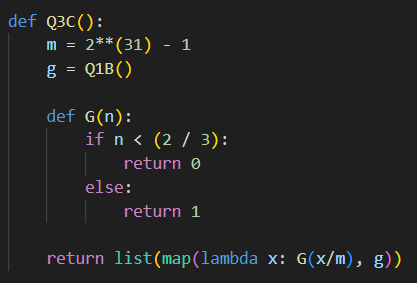
\includegraphics{Images/3C.png}
    \end{center}

    \item (1 point) Let $g(1),g(2), \ldots, g(10000)$ be the values you generated in Question 1 (c). Denote 
    \begin{align*}
        x_i=G\left(\frac{g(i)}{m}\right),\ \ \mbox{ for all }i=1,2,\ldots, 10000,
    \end{align*}
    where $m=2^{31}-1$. Plot and show the graph of the following function of $t$
    \begin{align*}
        \frac{1}{10000}\sum_{i=1}^{10000}\mathbf{1}\{x_i\le t\}.
    \end{align*}

    \begin{center}
        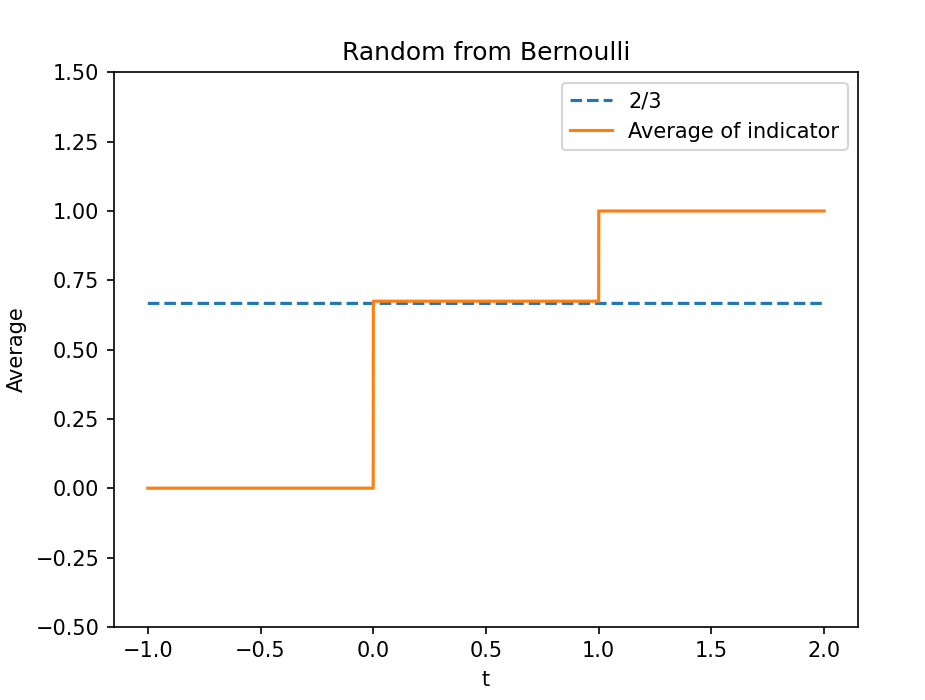
\includegraphics[width=0.6\textwidth]{Images/3D Plot.png} \quad 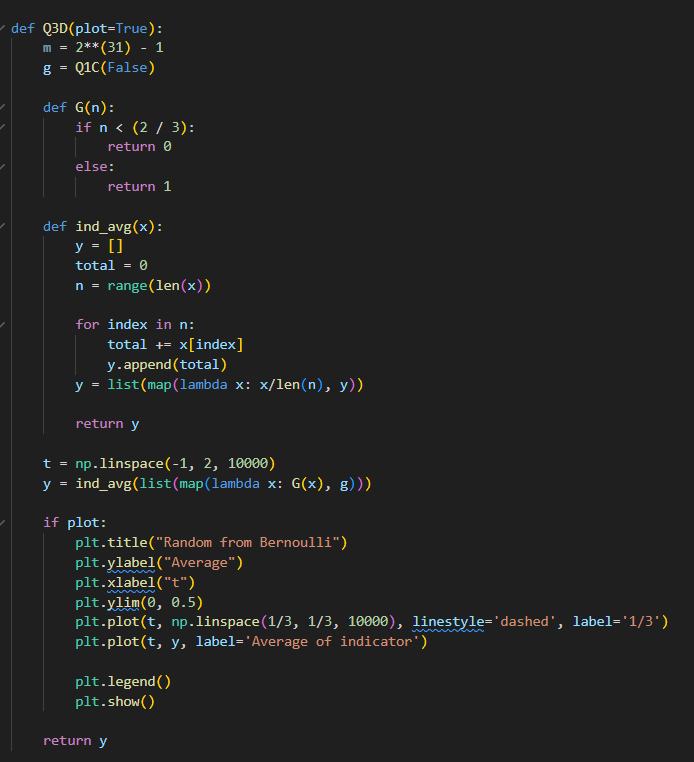
\includegraphics[width=0.6\textwidth]{Images/3D.png}
    \end{center}
\end{enumerate}



\end{enumerate}


\end{document}
